\documentclass[12pt,oneside,landscape,final]{memoir}

\usepackage{local}

\begin{document}

\title{Az Ülés Művészete}
\author{Ajahn Kalyāno}

\newlength{\foldmarkhoriz}
\setlength{\foldmarkhoriz}{\stockwidth}
\addtolength{\foldmarkhoriz}{-0.5pt}

\AddToShipoutPicture{%
\put(\LenToUnit{\foldmarkhoriz},\LenToUnit{0pt}){%
\color[gray]{0.5}\rule{1pt}{8mm}%
}%
\put(\LenToUnit{\foldmarkhoriz},\LenToUnit{202mm}){%
\color[gray]{0.5}\rule{1pt}{8mm}%
}%
}

\pagestyle{empty}
\setlength{\parindent}{0pt}
\setlength{\parskip}{0.6\baselineskip}

\mbox{}\vfill

{\centering
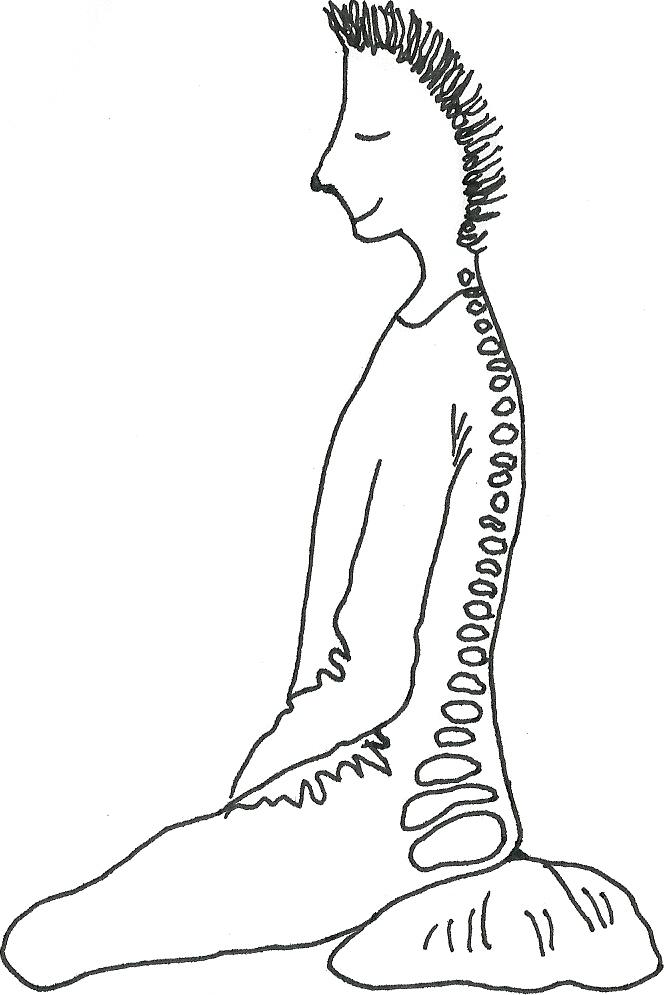
\includegraphics[keepaspectratio,width=80mm]{sitting-bones.jpg}
\par}

\vfill\mbox{}

\clearpage

\mbox{}\vfill

{\centering

Ajahn Kalyāno-nak az Amaravati Kolostor kiadásában megjelent alábbi kis írása az
ülésről szól. Ajahn Kalyāno 1961-ben született Angliában, és 17 éves kora óta
gyakorló buddhista. Világi hívőként gyakorlása részeként több mint 20 évet
dolgozott kórházakban, ahol klinikai pszichológusként, gyógytornászként és T’ai
Chi tanárként fő területei a neurológiai rehabilitáció és a tanulási
fogyatékosságok voltak. Mindig különös érdeklődéssel fordult a test és az elme
kapcsolatának megismerése felé. Ajahn Kalyāno-t 1995-ben a Chithurst Kolostorban
avatták szerzetessé.

}

\vfill\mbox{}

\clearpage

\mbox{}\vfill

{\centering

\includegraphics[keepaspectratio,width=80mm]{stones.jpg}
\par}

{\centering
{\Huge Az Ülés Művészete}

Ajahn Kalyāno
\par}

\vfill\mbox{}

\clearpage

Az ülőmeditációt évek óta a gyógytornász szemével is nézem, és sok embernek
segítettem már, hogy megoldjuk az üléssel kapcsolatos problémáikat. Érdemes
tudnunk, hogy a hátradőlés és támaszkodás nélküli ülésnek sokkal több fizikai
előnye van mint hátránya, és hogy ennek a képességnek az elsajátítása segíti a
testtudatosság kifejlesztését, ami sokak számára a legfontosabb eszköz a
vándorló elme megállításához.

Az üléssel kapcsolatos minden probléma amivel találkoztam, megelőzhető egyszerű
gyakorlatokkal és néhány dologra való odafigyeléssel.

\section{Helyes testtartás}

A helyes testtartást alulról kezdjük felépíteni. Ha helyesen alapozzuk meg az
ülésünket, akkor jobban tudjuk tartani a hátunkat és a nyakunkat is.
Használhatunk egy párnát arra, hogy azzal mint egy ékkel előredöntsük a
medencecsontunkat, és így egy előrehajló ívet hozzunk létre a gerinc alsó
részén.

A helyes testtartás, ami nem erőlteti a hátunkat, ez után nagyrészt azon múlik,
hogy megtanuljuk a hátunkat tartani elölről és hátulról is. Erős izmaink vannak,
amikkel elölről támasztva tudjuk a hátunkat egyenesen tartani: a hasizom, a nagy
horpaszizom és az egyenes combizom.

{\centering\par
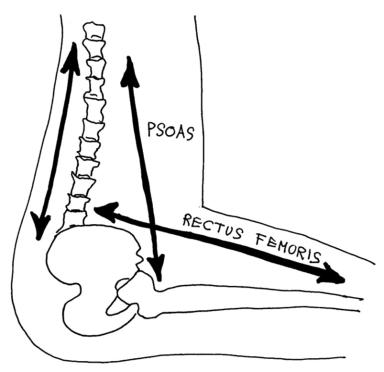
\includegraphics[keepaspectratio,width=50mm]{muscles-and-bones.jpg}
\par}

\clearpage

\section{Gyakorlatok}

Ennek a két testtartásnak gyakorlása segíthet minket abban, hogy helyesen
tudjunk ülni:

{\centering\par
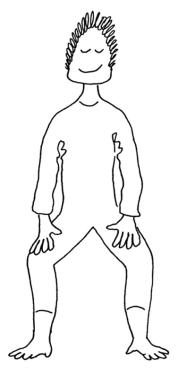
\includegraphics[keepaspectratio,height=50mm]{tai-chi-stand-1.jpg}%
\hspace*{5mm}%
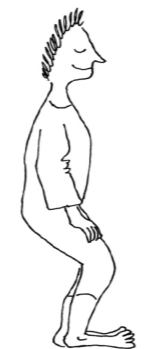
\includegraphics[keepaspectratio,height=50mm]{tai-chi-stand-2.png}
\par}

a) T’ai Chi állás – álljunk behajlított térdekkel, széttett lábakkal. Tartsuk ki
az állást amíg bírjuk, és fejlesszük ki, hogy legalább két percig tudjunk így
állni.

{\centering\par
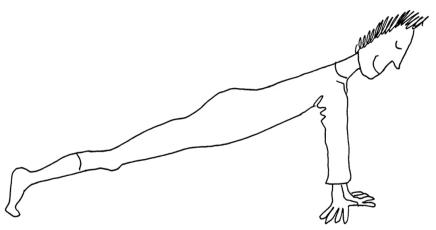
\includegraphics[keepaspectratio,height=30mm]{plank-stand.jpg}%
\par}

b) „palló” tartás a horpaszizmok erősítésére – tartsuk a testünket
fekvőtámaszban egyenesen amíg bírjuk, és fejlesszük ki, hogy legalább egy percig
tudjuk így tartani magunkat.

Idővel érezni fogjuk, hogy egy kicsit hátra tudunk dőlni ülés közben, hogy
kihasználjuk az így megerősödött izmaink segítségét.

\section{Fájdalom}

A térdben jelentkező fájdalmakat egyszerű nyújtásokkal tudjuk megelőzni.

\clearpage

Példaként egy nyújtógyakorlat: feküdjünk le, és tegyük egyik lábunkat keresztbe
a másikon:

{\centering\par
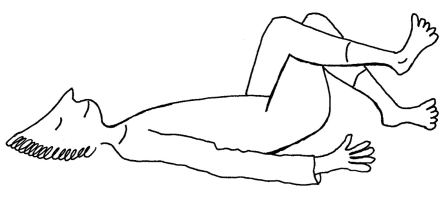
\includegraphics[keepaspectratio,width=48mm]{cross-one-leg.png}%
\par}

majd emeljük fel az alul lévő térdünket

{\centering\par
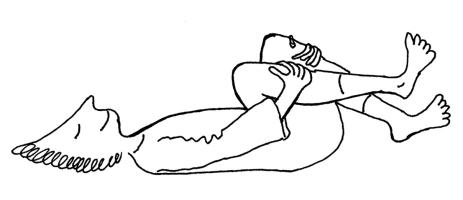
\includegraphics[keepaspectratio,width=48mm]{lift-the-knee.jpg}%
\par}

és hátra gördülve húzzuk lassan a mellünk felé, hogy a felül lévő lábunk oldalán
érezzük a feszültséget a fenekünk tájékán.

{\centering\par
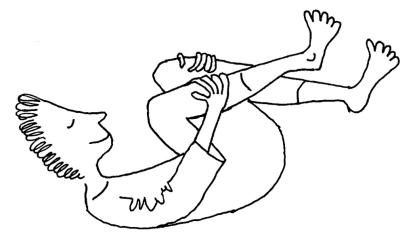
\includegraphics[keepaspectratio,width=48mm]{pull-toward-the-chest.jpg}%
\par}

Ha meditáció közben fél-lótusz pózban szoktunk ülni, akkor jó, ha rendszeresen
változtatjuk, hogy melyik lábat helyezzük felülre.

Ahhoz, hogy magabiztosan gyakorolhassunk tovább amikor megtapasztaljuk a test
határait, fontos tudnunk, hogy melyik fájdalom utal olyasmire, amiből sérülés
származhat, és melyik fájdalom nem utal sérülésre. Problémákra utalhatnak az
éles fájdalmak, és minden olyan fájdalom, ami nem múlik el azonnal, amikor
testtartást váltunk. Sokáig tartó mozdulatlan ülés során tapasztalhatunk tompa
fájdalmat, ezt azonban csökkenteni tudjuk azzal, hogy amennyire lehet, egyenesen
tartjuk testünket.

\end{document}
